\documentclass[12pt,fleqn]{article}

\usepackage{amsmath, amsthm, amssymb} %math expressions, theoreme/lemma, math symbols
\usepackage{mathtext} %russian letters in formulas

% fonts and lang
\usepackage{cmap}
\usepackage[T1, T2A]{fontenc}
\usepackage[utf8]{inputenc}
\usepackage[english, russian]{babel}

% formatting
\usepackage{geometry} %customize page layout
\geometry{left = 3cm}
\geometry{right = 1.5cm}
\geometry{top = 2cm}
\geometry{bottom = 2cm}

\usepackage{rotating}
\usepackage{minted}
\usepackage{mdframed}


\begin{document}
    \begin{titlepage}
        \begin{center}
            \textsf{\Large\bfseriesИнструкция к библиотеке QComputations}\\[15mm]
        \end{center}
    \end{titlepage}

    \newpage

    \setcounter{page}{2}
	\thispagestyle{empty}
	\tableofcontents

    \newpage

    \section{Введение}
        Данная инструкция призвана только научить пользователя использовать данную библиотеку. Квантовая теория будет здесь описана очень кратко, подразумевается, что вы её уже знаете. 
        Также здесь не рассказываются детали реализации библиотеки. Это можно найти в \textsf{documentation.pdf}.

        Библиотека призвана решить 4 цели:
        \begin{enumerate}
            \item{Избавить программиста от нужды реализовывать всё необходимое для квантовых вычислений, в том числе и математические абстракции.}
            \item{Программист должен думать исключительно в нотациях квантовой механики, то есть в нотациях формул и физических абстракций.}
            \item{Библиотека, в силу экспоненциального роста сложности вычислений и требуемой памяти, должна быть полностью распараллелена. 
            На данный момент \textbf{QComputations} полностью совместима с Ломоносов-2 (МГУ-270).
             Версия конкретно для Ломоносов-2 лежит в закрытом доступе из соображений безопасности.}
            \item{Квантовые вычисления так устроены, что при некорректных формулах, функциях или константах, может получиться правдободный ответ, то есть по результату зачастую в принципе 
            нельзя сказать, есть ли ошибка в программе или нет. \textbf{QComputations} призван сильно уменьшить вероятность подобных ошибок.}
        \end{enumerate}

        Вся библиотека работает на базе программного пакета с открытым исходным кодом - \textsf{Intel OneAPI}. 
        Документация к этой библиотеке безумно сложна, содержит неточности, недосказанности и ошибки. 
        
        Компиляция происходит также с их компиляторами - \textsf{icpx} и \textsf{mpiicpx}
        (для чуть более старых версий \textsf{Intel Oneapi} - \textsf{icpc} и \textsf{mpiicpc}).

        Пример компиляции:

\begin{mdframed}[linecolor=black, topline=true, bottomline=true,
    leftline=false, rightline=false]
\begin{minted}[mathescape]{bash}
icpx filename.cpp -ldl -lQComputations_SINGLE
\end{minted}
\end{mdframed}

         \textbf{QComputations} избавляет от надобности вникать в данный загромждённый пакет. В будущем будет версия на \textsf{CUDA}, что даст возможность в принципе его не использовать.

        Вся инструкция поделена на 8 частей.
        \begin{enumerate}
            \item{\textbf{Матрицы}: Сначала мы начнём с использования базовых математических классов - матриц. В библиотеке их 2: обычная и блочно-распределённая.
        Блочно-распределённая работает на сетке \textsf{BLACS} - идея Intel. Данная часть по своей сути описывает принципы её работы, так как всё остальное элементарно.}
            \item{\textbf{QConfig}: Здесь объяснено, как работать с конфигуратором всей библиотеки.}
            \item{\textbf{Базисное состояние и суперпозиция}: Мы разберём основу всей библиотеки (структура \textbf{QComputations}
             графически изображена в \textsf{documentation.pdf}) - базисное состояние.}
            \item{\textbf{Операторы}: Объясняется, как писать собственные операторы.}
            \item{\textbf{Гамильтониан}: Объясняется, как работать с гамильтонианом и как писать собственные.}
            \item{\textbf{Моделирование}: Объясняется, как моделируется эволюция состояний под воздействием гамильтониана.}
            \item{\textbf{Визуализация}: Объясняется, как визуализировать результаты и кастомизировать графики.}
            \item{\textbf{Инструкция к параллелизации}: Здесь даются некоторые советы по работе с данной библиотекой. (Возможно здесь вы найдёте ответы,
            почему у вас может что-то не работать, или работать очень медленно.)}
        \end{enumerate}

        \section{Матрицы}
        Как ни покажется странным, одна из главных причин, почему пришлось написать собственные классы матриц (помимо банального удобства) - это странная реализация \textsf{Intel OneAPI},
        а точнее его блочного распределения. Дело в том, что пакет написан на Fortran, а в нём 
        матрицы хранятся по столбцам (в C хранятся по строкам). Одноядерная версия (обычный Lapack и blas) поддерживают оба стиля хранения матриц, но вот распределённые же аналоги (scalapack и 
        pblas) поддерживают исключительно стиль Fortran. Собственно, в \textbf{QComputations} матрицы/блоки могут переключаться между этими стилями.

        Классы называются \textbf{Matrix<T>} и \textbf{BLOCKED\_Matrix<T>}. Для них реализованы всевозможные операторы, операции над матрицами и полезные функции. 
        Хранить можно любой тип данных, но операторы работают только для \textbf{double} и \textbf{std::complex<double>}. 
        Главное же преимущество этих двух классов - это их абсолютная схожесть. Как было сказано, одно из 
        целей библиотеки, чтобы программист в принципе не думал о её реализации. Если вы хотите перейти от обычной матрицы к блочной распределённой - вам нужно сделать всего лишь две вещи.

        \begin{enumerate}
            \item{инициализировать сетку \textsf{BLACS} (про неё чуть позднее), что можно сделать одной командой \textbf{init\_grid(ctxt)}}
            \item{Поменять название класса \textbf{Matrix<T>} на \textbf{BLOCKED\_Matrix<T>}, вставив результат \textbf{ctxt} в 1 аргумент}
        \end{enumerate}

        Поздравляю, теперь ваша матрица полностью блочно распределена. И все те математические формулы, функции и операции абсолютно аналогичны базовой матрице \textbf{Matrix<T>}.
        Также, очевидно, работает и в обратную сторону.

        Оба этих класса поддерживают множество конструкторов (способов генерации), все их можно посмотреть в документации.

        Поговорим теперь о сетке \textsf{BLACS} о её влиянии на \textbf{BLOCKED\_Matrix<T>} и на производительность.
        Данная сетка устроена не совсем интуитивно, дело в том, что её блоки устроены циклично. Авторы \textsf{Intel OneAPI} хотели сделать алгоритм распределения блоков таким образом,
         чтобы под него подходило любое число процессов, любые размеры блоков и так далее. Объясню теперь само устройство сетки на примерах:

        Возьмём матрицу например 5 на 5 - 
        $$
        \begin{bmatrix}
        1 & 2 & 3 & 4 & 5\\
        6 & 7 & 8 & 9 & 10\\
        11 & 12 & 13 & 14 & 15\\
        16 & 17 & 18 & 19 & 20\\
        21 & 22 & 23 & 24 & 25
        \end{bmatrix}
        $$

        Допустим у нас теперь есть сетка процессов - то есть их абстрактное расположение между собой.
        В качестве примера также возьмём сетку 2 на 2 (соответственно 4 ядра):

        Тогда сетка будет следующей:

        $$
        \begin{pmatrix}
        0 & 1\\
        2 & 3
        \end{pmatrix}
        $$

        где номера - ранги ядер.

        Теперь возьмём размеры базовых блоков (\textbf{NB} и \textbf{MB}) равными 2 на 2. Тогда распределение будет следующим:

        $$
        0: \begin{bmatrix}
           1 & 2 & 5\\
           6 & 7 & 10\\
           21 & 22 & 25
           \end{bmatrix}
        1: \begin{bmatrix}
            3 & 4\\
            8 & 9\\
            23 & 24
            \end{bmatrix}
        2: \begin{bmatrix}
            11 & 12 & 15\\
            16 & 17 & 20
            \end{bmatrix}
        3: \begin{bmatrix}
            13 & 14\\
            18 & 19
            \end{bmatrix}
        $$

        Как видно, распределение здесь циклично.
        
        Про генерацию должен сказать, что поддерживается 3 вида матриц. GE - общего вида, SY - симметрическая, HE - эрмитовая. Как ни покажется странным, SY и HE не дают экономию памяти,
         для них просто не инициализируются элементы нижнетреугольной части (причём обязательно!).

        \section{QConfig}
        Одной из проблем квантовых вычислений - это огромное число констант, зависящих друг от друга. Слежка за ими всеми в огромной программе для хорошего программиста не проблема,
         но здесь всё омрачает сама квантовая физика, которая выглядит правдоподобной при любых константах, но к реальности будут иметь отношения лишь конкретные, подчиняющиеся строгим формулам.

         Изначально, данный конфигуратор предназначался исключительно для них, впоследствии эта идея оказалась куда удобней, чем на 1 взгляд, поэтому теперь с её помощью можно настраивать всю 
         библиотеку в целом: алгоритмы, поведения библиотеки, размеры ячеек возвращаемых CSV файлов и так далее, подробнее в документации.

        Приведу примеры:

        Допустим мы хотим увеличить точность (число цифр после запятой) результатов при записи в CSV файлы. По умолчанию данное значение стоит - 16. Чтобы его изменить, можно написать следующее:

\begin{mdframed}[linecolor=black, topline=true, bottomline=true,
    leftline=false, rightline=false]
\begin{minted}[mathescape]{c++}
QConfig::instance().set_csv_num_accuracy(new_accuracy);
\end{minted}
\end{mdframed}

        И всё, теперь при матрицы в CSV файл будут записаны с новой точностью.

        \section{Базисное состояние}
        
        Теперь перейдём уже к самой библиотеке с точки зрения квантовых вычислений. Сложность написания хорошей библиотеки для данной цели в том, что в квантовой теории абсолютно всё 
        взаимосвязано, то есть нет, как в математике, некоторых понятия, которые оборачиваются в другие понятия, потом ещё в одни и так далее, то есть невозможно квантовую механику математически 
        описать последовательно.
        Ранняя версия опиралась на понятие оператора. Как оказалось, такое решение не может похвастаться гибкостью из-за того, 
        что с операторами неудобно описывать состояния. Данная же версия полностью опирается на понятие состояния, и как оказалось,
        данная идея на практике позволяет с лёгкостью описывать любые системы.

        Начнём с простого, базисное состояние $|\Psi\rangle$ - это обычный вектор из кудитов (многозначных кубитов). Пример состояния $|12,3,0\rangle|11,2\rangle$.
         Для примера я показал ещё понятие ``групп'' - объединение некоторых кубитов друг с другом, это бывает удобно для описания операторов, но подробнее мы этом затронем при объяснении в самих операторах.
        Каждый кудит имеет своё максимальное значение. Базисное состояние - это не то состояние в привычном смысле, а лишь одно конкретное (физическое), а точнее то, которые мы можем получить в результате 
        измерения. В книгах по квантовой информатике они обозначаются как $|0\rangle$ и $|1\rangle$, в физике, например для поляризации фотона - $|H\rangle$ и $|V\rangle$. Также, нужно помнить, что каждая
        абстракция привязана к какому-то базису, который, в свою очередь, как-то отсортирован, то есть, абсолютно везде должна быть одна и та же сортировка (эту задачу на себя берёт полностью библиотека).

        Из вышеперечисленного мы и получаем, что для такого класса нам необходимо помнить максимальное значение для каждого кудита, объединять их в группы, хранить сами значения кудитов и задавать 
        правила сортировки.

        Всё это реализовано в классе \textbf{Basis\_State}. Сортировка там реализована в обратном порядке по строковому представлению, но её можно будет перегрузить.
        При проектировании собственного понятия состояния нужно помнить всю структуру класса \textbf{Basis\_State} и то, как с ним работать, а точнее - то, что он хранит.

\begin{mdframed}[linecolor=black, topline=true, bottomline=true,
    leftline=false, rightline=false]
\begin{minted}[mathescape]{c++}
class Basis_State {
    public:
        // инициализация пустого состояния
        explicit Basis_State() = default;

        // groups_count делит кудиты на равные по размеру группы.
        // max_val - максимальное значение всех кудитов
        explicit Basis_State(size_t qudits_count, ValType max_val = 1,
                                size_t groups_count = 1);

        // добавление поддержки для разных кудитов. 
        // max_vals - вектор, в котором для каждого кубита
        // указано его максимальное значение.
        explicit Basis_State(size_t qudits_count, 
                            const std::vector<ValType>& max_vals,
                            size_t groups_count = 1);

        // qudit_count - чилсо кудитов. 
        // max_val - максимальное значение их всех. 
        // groups - количество элементов в каждой группе. 
        // В сумме должно получиться qudits_count, иначе ошибка.
        // ВНИМАНИЕ!!! - groups потом хранится в другом виде. 
        // А именно, в нём хранятся индексы последних кудитов групп. 
        // Так сделано в целях удобства индексации.
        // Например, для |10>|001> вектор groups_ = {1, 4}
        // Для ориентации в данном векторе сделаны отдельные методы,
        // приведённые ниже
        explicit Basis_State(size_t qudits_count, ValType max_val, 
                                const std::vector<size_t>& groups);

        // ====== Далее идут варианты с иницализацией значений ========

        // Создания состосния с инициализацией значений
        explicit Basis_State(const std::vector<ValType>& qudits, 
                                ValType max_vals = 1, 
                                size_t groups_count = 1);

        // Создание состояния с инициализация значений с поддержкой разных кудитов
        explicit Basis_State(const std::vector<ValType>& qudits,
                                const std::vector<ValType>& max_vals,
                            size_t groups_count = 1);

        // Создание состояния с инициализация значений
        // с поддержкой разных кудитов + разных групп
        explicit Basis_State(const std::vector<ValType>& qudits, 
                                const std::vector<ValType>& max_vals,
                            const std::vector<size_t>& groups_sizes);

        // Инициализация вектора через строку формата |0;1>|2>
        // max_vals - максимальное значение для всех кудитов
        explicit Basis_State(const std::string& qudits, ValType max_vals = 1);
        // max_vals - максимальное значение для каждого кудита
        explicit Basis_State(const std::string& qudits, const std::vector<ValType>& max_vals);

        // Установить состояние через строку формата |0;1>|2>
        void set_state(const std::string& str_state);

        // Установить кудиту значение. 
        // qudit_index - индекс кудита. 
        // group_id - номер группы (нумерация с нуля)
        void set_qudit(ValType val, size_t qudit_index, size_t group_id = 0);
        // Получить значение кудита
        ValType get_qudit(size_t qudit_index, size_t group_id = 0);

        // Добавить кудит. Будет добавлен к последней группе
        void append_qudit(ValType init_val = 0, ValType max_val = 1);

        // Проверка, является ли состояние пустым
        bool is_empty();

        // Возвращает число кудитов в системе
        size_t qudits_count() const { return qudits_.size();}

        // Получить индексы последних кудитов групп
        std::vector<size_t> get_groups();

        // Получить индекс начала группы
        size_t get_group_start(size_t group_id);

        // Получить индекс конца группы 
        // (Например |10>|10> для 0 группы индекс конца будет 1)
        size_t get_group_end(size_t group_id);

        // Получить число групп
        size_t get_groups_count();

        // Получить размер  группы
        size_t get_group_size(size_t group_id);

        // Получить в качестве состояния отдельную группу
        Basis_State get_group(size_t group_id) const;

        // Установить группу через строку формата |0;1>
        // index_start - индекс начала строкового
        // представления группы в строке
        // Например в примере |0;1>|2> index_start группы |2> равен 5
        void set_group(size_t group_id, const std::string& group_str,
                       size_t index_start = 0);

        // Конвертировать состояние в строку
        // Перегружаемый метод (виртуальный)
        virtual std::string to_string() const;

        // Выдаст ошибку, если состояния различаются по группам
        // или по максимальным значениям кудитов
        bool operator==(const Basis_State& other);
        // Оператор сравнения можно перегрузить
        virtual bool operator<(const Basis_State& other);
        
        // Поменять максимальное значение кудита
        void set_max_val(ValType val, size_t qudit_index, size_t group_id = 0);
        // Получить максимальное значение кудита
        ValType get_max_val(size_t qudit_index, size_t group_id = 0);
        // Получить вектор максимальных значений
        std::vector<ValType> max_vals();

        // Получить индекс состояния в базисе
        size_t get_index(const std::set<Basis_State>& basis) const;

        // Очистить состояние
        void clear() { qudits_.resize(0); max_vals_.resize(0); groups_.resize(0); }
    protected:
        std::vector<ValType> qudits_; // Вектор кудитов
        std::vector<ValType> max_vals_; // Вектор максимальных значений кудитов
        std::vector<size_t> groups_; // Вектор конца групп
};

\end{minted}
\end{mdframed}

        Разберём подробнее. \textbf{Basis\_State} по своей сути хранит 3 вещи:
        \begin{itemize}
            \item{\textbf{qudits\_} - собственно значения кудитов}
            \item{\textbf{max\_vals\_} - максимальные значения кудитов (минимальное значение - 0)}
            \item{\textbf{groups\_} - позволяет объединять кудиты в группы. Хранит индексы конца каждой группы. Среди методов \textbf{Basis\_State} есть методы для удобной индексации между ними}
        \end{itemize}

        Давайте создадим базисное состояние - $|0;1;2\rangle|1;0>$. Пример - \textsf{basis\_state.cpp}.

\begin{mdframed}[linecolor=black, topline=true, bottomline=true,
leftline=false, rightline=false]
\begin{minted}[mathescape]{c++}
using namespace QComputations;

Basis_State state(5, 1, {3, 2});

state.set_qudit(1, 1, 0);
state.set_max_val(2, 2, 0);
state.set_qudit(2, 2, 0);
state.set_qudit(1, 0, 1);

std::cout << "SET_MANUALLY: " << state.to_string() << std::endl;
// |0;1;2>|1;0>

Basis_State new_state(8, 4, 4);
new_state.set_state("|4;2>|1;1>|3;2>|1;2>");

std::cout << "SET_STATE: " << new_state.to_string() << std::endl;
// |4;2>|1;1>|3;2>|1;2>

new_state.set_group(2, "|0;0>");

std::cout << "SET_GROUP: " << new_state.to_string() << std::endl;
// |4;2>|1;1>|0;0>|1;2>
\end{minted}
\end{mdframed}


        \subsection{Создание произвольного базисного состояния}

        Теперь к вопросу, как сделать собственное понятие состояние. А очень просто - сделать дочерний класс для \textbf{Basis\_State}, добавив к нему необходимые функции и данные. Разберём на примере 
        состояния для описания системы Тависа-Каммингса (оптическую полость из 1 полости и множества атомов). Пример описан для одноядерной версии - \textsf{realization\_tc\_example.cpp},
         и для блочной - \textsf{blocked\_realization\_tc\_example.cpp}. 

\begin{mdframed}[linecolor=black, topline=true, bottomline=true,
leftline=false, rightline=false]
\begin{minted}[mathescape]{c++}
class TC_State : public Basis_State {
public:
    // нулевой кудит - число фотонов,
    // остальные - состояния атомов
    // m - число атомов
    explicit TC_State(int m,
                        int n = 0) :
                Basis_State(m + 1) {
        this->set_max_val(std::max(QConfig::instance().max_photons(), n),
                            0);
        this->set_qudit(n, 0);
    }

    // Инициализация с помощью строки
    explicit TC_State(const std::string& str) :
        Basis_State(str) {
        this->set_max_val(std::max(QConfig::instance().max_photons(), 1),
                        0);
    }

    // Инициализировать состояние по строке
    // Формат (пример - |0;1>|3;14;1>) ПОЛНОСТЬЮ совпадает с Basis_State
    // Его изменение подразумевает переписывание конструктора, 
    // или владения регулярными выражениями, что является 
    // необычным навыком для квантовых вычислений, 
    // поэтому к формату проще привыкнуть.
    explicit TC_State(const std::string& str) :
        Basis_State(str) {
        this->set_max_val(std::max(QConfig::instance().max_photons(), 1),
                            0);
    }


    // установить число фотонов
    void set_n(int n) {this->set_qudit(n, 0);}
    // получить число фотонов
    int n() const { return this->get_qudit(0);}
    // получить число атомов
    int m() const { return this->qudits_count() - 1;}

    // установить максимальное число фотонов
    void set_max_photons(int max_photons) {
        this->set_max_val(max_photons, 0);    
    }

    // установить значение атому
    void set_atom(int val, size_t qudit_index = 0) { 
        this->set_qudit(val, qudit_index + 1);
    }

    // получить значение атома
    int get_atom(size_t qudit_index = 0) const { 
        return this->get_qudit(qudit_index + 1);
    }

    // установить интенсивность утечки фотонов
    void set_leak(double leak) { leak_ = leak; }
    // получить интенсивность утечки фотонов
    double get_leak() const { return leak_;}

    // установить интенсивность притока фотонов
    void set_gain(double gain) { gain_ = gain;}
    // получить интенсивность притока фотонов
    double get_gain() const { return gain_;}

    // установить силу взаимодействия электронов
    // с фотонами
    void set_g(double g) { g_ = g;}
    double g() const { return g_;}

    // перегрузка вывода состояния в строку
    std::string to_string() const override;

    // перегрузка сортировки
    // ОБРАЩАЮ ВНИМАНИЕ! Перегружается с аргументом 
    // const Basis_State&
    bool operator<(const Basis_State& other) const override {
        TC_State* b = (TC_State*)(&other);

        if (this->n() < b->n()) return false;
        else if (this->n() == b->n()) {
            for (size_t i = 0; i < this->m(); i++) {
                if (this->get_atom(i) < b->get_atom(i)) return false;
                else if (this->get_atom(i) > b->get_atom(i)) return true;
            }
        }

        return true;
    }
private:
    double leak_; // Интенсивность утечки фотонов
    double gain_; // Интенсивность притока фотонов
    double g_ = QConfig::instance().g(); // Сила взаимодействия электронов с полем
};

std::string TC_State::to_string() const {
    auto res = this->Basis_State::to_string();
    size_t start_pos = 0;
    int index = 1;
    while((start_pos = res.find(";", start_pos)) != std::string::npos) {
        res[start_pos++] = (index > 0 ? ';' : ',');
        index--;
    }

    return res;
}

\end{minted}
\end{mdframed}

        \textbf{Резюмирую}: чтобы сделать собственное понятие состояния, нужно инициализировать дочерний класс \textbf{Basis\_State},
        а дальше реализовать всё то, что вам необходимо для работы с вашей абстракцией. Также возможна перегрузка строкового представления, а также сортировки.

        \subsection{Суперпозиция}

        Теперь о том, как сделать суперпозицию состояний. В библиотеке реализован шаблонный класс - \textbf{State<StateType>}. На вход к нему вы можете просто подать любое базисное состояние - появится 
        суперпозиция из 1 базисного состояния с единичным коэффициентом. Предупреждаю, вектор \textbf{не} нормализуется автоматически, для этого сделан отдельный метод \textbf{normalize()}.

        Давайте создадим суперпозицию двух состояний - $|00\rangle$ и $|11\rangle$, причём как нормированную, так и нет.

        Пример - \textsf{basis\_state.cpp}.
\begin{mdframed}[linecolor=black, topline=true, bottomline=true,
leftline=false, rightline=false]
\begin{minted}[mathescape]{c++}
// Создаём базисные состояния
Basis_State zero("|0;0>", 1);
Basis_State one("|1;1>", 1);

// Инициализация State<Basis_State>
State<Basis_State> st(zero);
st += one;
st *= 2;

std::cout << "State<Basis_State>: " << st.to_string() << std::endl;
// 2 * |0;0> + 2 * |1;1>

st.normalize();

std::cout << "State<Basis_State> NORMALIZE: " << st.to_string() << std::endl;
// (|0;0> + |1;1>)/sqrt(2)

// Теперь, если мы хотим добавить в базис суперпозиции состояние,
// но не хотим присваивать ему какой-либо коэффициент, 
// тогда метод insert
Basis_State zero_one("|0;1>", 1);
// Add state in basis of State<Basis_State>, but with coefficient = 0
st.insert(zero_one);

std::cout << "State<Basis_State> + zero_one: " << st.to_string() << std::endl;
// (|0;0> + |1;1>)/sqrt(2) + 0*|0;1>

\end{minted}
\end{mdframed}
        \section{Операторы}

        Перейдём теперь к фундаменту всей квантовой теории - операторам. Операторы в квантовой механики разные: операторы эволюции (унитарные эрмитовые матрицы), наблюдаемые (эрмитовые матрицы), 
        обычные операторы (вытекающие из физики, например операторы создания и уничтожения фотонов). Их все можно описать с помощью матриц, но на практике, этот способ требует безумное количество памяти, 
        очень трудозатратный и ведёт с большой вероятностью к тяжело распознаваемым ошибкам.
        Более того, некоторые из них описывают некоторые простое действие, например оператор уничтожения фотонов:
        $a|n\rangle = \sqrt(n)|n - 1\rangle$, и для подобных операторов неудобно использовать матрицы как абстракции для их инициализации.
        Цель класса операторов в этой библиотеке - дать возможность описать его действие простой функцией. 
        Вы можете в неё засунуть также и матрицу в чистом виде с помощью некоторой глобальной функции (чего я делать 
        крайне не рекомендую), но всё же чаще, вы будете просто описывать формальное действие этого оператора. Более того, данное решение позволяет оптимизировать реализацию формул, например, объединить 
        сумму операторов абстрактно в один оператор, и написать оператор, описывающий действией всей этой суммы. Дальше будут примеры подобного.

        В библиотеке для всего этого реализован класс \textbf{Operator<StateType>}. 
        Общий вид функции, которую необходимо реализовать для описания действия оператора выглядит следующим образом:

\begin{mdframed}[linecolor=black, topline=true, bottomline=true,
leftline=false, rightline=false]
\begin{minted}[mathescape]{c++}
State<StateType> op_func(const StateType& state) {
    // do something
    // return State<StateType> res
}
\end{minted}
\end{mdframed}
        То есть, это функция, на вход которой подаётся некоторое базисное состояние, а на выход вы получаете суперпозицию состояний. Глобально, это всё.
        Вы можете дальше суммировать операторы следующим образом:

\begin{mdframed}[linecolor=black, topline=true, bottomline=true,
leftline=false, rightline=true]
\begin{minted}[mathescape]{c++}
//a_i - комплексные числа
using OpType = Operator<Some_State>;
OpType H = OpType(some_op_1_1) * OpType(some_op_1_2) * ... * 
           OpType(some_op_1_n) * a_1 + 
           OpType(some_op_2_1) * OpType(some_op_2_2) * ... *
           OpType(some_op_2_n) * a_2 +
           ...
           OpType(some_op_m_1) * OpType(some_op_m_2) * ... *
           OpType(some_op_m_n) * a_m;
\end{minted}
\end{mdframed}
    
        Потом прогонять через них суперпозицию состояний методом \textbf{run} (а также умножение и оператором \textbf{()}).

        Теперь давайте разберёмся, а как их собственно создавать.

        \subsection{Вспомогательные функции для создания собственных операторов}
        Как было сказано в \textbf{Basis\_State}, метод \textbf{set\_qudit}, если ему передать значение больше максимального, то будет выдана ошибка. Для операторов декогеренции (и не только для них) это 
        является проблемой, так как, например, для притока фотонов, кудитов для фотонов может улетать в бесконечность, а постоянно проверять неудобно, к тому же мы работаем с базисным состояниями, а 
        не с суперозицией. Собственно, для решения этих неудобств и были написаны эти функции.

        \begin{center}
            \textbf{set\_qudit} - установка значения кудиту.
        \end{center}

        Устанавливает значению кудиту - на выход получаете данное состояния в виде \newline \textbf{State<StateType>} с единичным коэффициентом.
         В случае, если устанавливается значения >= максимальному значению кудита, то в ответ возвращается пустое состояние, то есть пустой \textbf{State<StateType>}.
        Собственно, для этого и нужны максимальные значения.

\begin{mdframed}[linecolor=black, topline=true, bottomline=true,
leftline=false, rightline=false]
\begin{minted}[mathescape]{c++}
// state - базисное состояние
// val - значение, которое мы устанавливаем
// qudit index - индекс кудита в группе
// group_id - номер группы, в котором находится кудит

template<typename StateType>
State<StateType> set_qudit(const StateType& state,
                           ValType val,
                           size_t qudit_index = 0,
                           size_t group_id = 0) {
    auto res = state; // копируем состояние

    // проверяем, принадлежит ли val диапазону от 0 до максимального значения
    if (val > state.get_max_val(qudit_index, group_id) or val < 0) {
        res.clear(); // очистить состояние
    } else {
        // устаналиваем значение кудита
        res.set_qudit(val, qudit_index, group_id);
    }

    // возвращаем результате в виде State<StateType>
    return State<StateType>(res);
}
\end{minted}
\end{mdframed}

        \begin{center}
            \textbf{get\_qudit} - получить значения кудита.
        \end{center}

        Возвращает переданное в функцию состояние в виде \textbf{State<StateType>} с коэффициентом, равным значению запрашиваемого кудита.

\begin{mdframed}[linecolor=black, topline=true, bottomline=true,
leftline=false, rightline=false]
\begin{minted}[mathescape]{c++}
// state - базисное состояние
// qudit index - индекс кудита в группе
// group_id - номер группы, в котором находится кудит

template<typename StateType>
State<StateType> get_qudit(const StateType& state,
                           size_t qudit_index = 0,
                           size_t group_id = 0) {
    auto res = State<StateType>(state); // привести состояние к
                                        // State<StateType>

    // Сделать коэффицент равным значению запрашиваемого кудита
    res[0] = state.get_qudit(qudit_index, group_id);

    return res;
}
\end{minted}
\end{mdframed}

        \begin{center}
            \textbf{sigma\_x, sigma\_y, sigma\_z} - операторы Паули.
        \end{center}

        Операторы Паули. Напомню, что операторы Паули выглядят следующим образом:

        $$
        {\sigma}_{x} = \begin{bmatrix}
                    0 & 1\\
                    1 & 0
                    \end{bmatrix}
        \sigma_{y} = \begin{bmatrix}
                    0 & -i\\
                    i & 0
                    \end{bmatrix}
        \sigma_{z} = \begin{bmatrix}
                    1 & 0\\
                    0 & -1
                    \end{bmatrix}
        $$
        
        Внутри реализована проверка на соответсвие значения кудитов. В случае, если кудит будет иметь некорректное значение - программа завершится с ошибкой.

\begin{mdframed}[linecolor=black, topline=true, bottomline=true,
leftline=false, rightline=false]
\begin{minted}[mathescape]{c++}
// state - базисное состояние
// qudit index - индекс кудита в группе
// group_id - номер группы, в котором находится кудит

template<typename StateType>
State<StateType> sigma_x(const StateType& state,
                         size_t qudit_index = 0,
                         size_t group_id = 0) {
    StateType res = state;
    auto qudit = state.get_qudit(qudit_index, group_id);
    assert(qudit == 0 or qudit == 1);

    if (qudit == 0) qudit = 1;
    else qudit = 0;

    res.set_qudit(qudit, qudit_index, group_id);

    return State<StateType>(res);
}

template<typename StateType>
State<StateType> sigma_y(const StateType& state,
                         size_t qudit_index = 0,
                         size_t group_id = 0) {
    StateType res = state;
    auto qudit = state.get_qudit(qudit_index, group_id);
    assert(qudit == 0 or qudit == 1);

    if (qudit == 0) { 
        qudit = 1;
    } else {
        qudit = 0;
    }

    res.set_qudit(qudit, qudit_index, group_id);

    State<StateType> stateres(res);
    stateres[0] *= COMPLEX(0, std::pow(-1, qudit + 1));

    return stateres;
}

template<typename StateType>
State<StateType> sigma_z(const StateType& state,
                         size_t qudit_index = 0,
                         size_t group_id = 0) {
    auto res = get_qudit(state, qudit_index, group_id);
    auto qudit = state.get_qudit(qudit_index, group_id);
    assert(qudit == 0 or qudit == 1);

    if (qudit == 1) {
        res[0] *= -1;
    }

    return res;
}
\end{minted}
\end{mdframed}

        \begin{center}
            \textbf{check} - оператор проверки значения кудиту. \newline
            \textbf{check\_func} - оператор проверки условия состояния через булевую функцию.
        \end{center}

        В некоторых задачах может возникнуть такая ситуация, что операторы работают только при определённом условии, то есть при определённых значениях кудита.
        Данный оператор проверяет значение указанного кудита - если значение подходит под условие, тогда оператор возвращает \textbf{State<StateType>} с единичным коэффициентом, 
        в противном случае возвращает пустое состояние. \textbf{check\_func} позволяет создавать условия любого вида для любого базисного состояния.

\begin{mdframed}[linecolor=black, topline=true, bottomline=true,
leftline=false, rightline=false]
\begin{minted}[mathescape]{c++}
// state - базисное состояние
// check_val - проверить кудит на равенство значению check_val
// qudit index - индекс кудита в группе
// group_id - номер группы, в котором находится кудит

template<typename StateType>
State<StateType> check(const StateType& state,
                       ValType check_val,
                       size_t qudit_index = 0,
                       size_t group_id = 0) {
    auto res = state;
    if (res.get_qudit(qudit_index, group_id) != check_val) {
        res.clear();
    }

    return State<StateType>(res);
}

//func - булевая функция проверки

template<typename StateType>
State<StateType> check_func(const StateType& state,
                       const std::function<bool(const StateType&)>& func) {
    auto res = state;
    if (func(state)) {
        res.clear();
    }

    return State<StateType>(res);
}
\end{minted}
\end{mdframed}

        \section{$H_{TC}$}

        Давайте реализуем все операторы, необходимые для гамильтониана Тависа-Каммингса.

        Формула $H_{TC} = \hbar{w_{ph}}{a^{\dagger}}{a} + {\hbar}{w_{at}}{\sum\limits_{i = 1}^{m}(\sigma^{\dagger}_{i}\sigma_{i})}
		+ {g}\sum\limits_{i=1}^{m}({a}\sigma^{\dagger}_{i} + a^{\dagger}\sigma_{i})$

        Реализуем 2 способами:
        \begin{enumerate}
            \item{Дословно}
            \item{Оптимизировано}
        \end{enumerate}

        \subsection{Дословная реализация $H_{TC}$}

        Как мы видим по формуле, такие операторы как $\sigma_{i}$ для каждого индекса по своей сути уникальный, так как он применяется к разным кубитам.
        В квантовой механике нет параметрических операторов, более того, даже если бы и были, не совсем понятно, как их делать универсальными и задавать в виде формул,
        с учётом всех свойств линейных операторов, так ещё эффективными и удобными. Чем-то, да придётся пожертвовать. 
        Но я покажу как даже, учитывая их отсутствие, дословно задавать подобные операторы в C++ с помощью лямбда-захвата. Пример - \textsf{accurate\_realization\_tc\_example.cpp}.

        Реализуем сначала операторы для создания и уничтожения фотонов. Так как они у нас применяются лишь к 1 кубиту, мы можем написать в обычном виде.
\begin{mdframed}[linecolor=black, topline=true, bottomline=true,
leftline=false, rightline=false]
\begin{minted}[mathescape]{c++}
//a|n> = sqrt(n)|n-1>
State<TC_State> a_destroy(const TC_State& st) {
    return set_qudit(st, st.n() - 1, 0) * std::sqrt(st.n());
}

//a+|n> = sqrt(n+1)|n+1>
State<TC_State> a_create(const TC_State& st) {
    return set_qudit(st, st.n() + 1, 0) * std::sqrt(st.n() + 1);
}
\end{minted}
\end{mdframed}

        Теперь реализуем оставшееся вместе с гамильтонианом.

\begin{mdframed}[linecolor=black, topline=true, bottomline=true,
leftline=false, rightline=false]
\begin{minted}[mathescape]{c++}
int main(int argc, char** argv) {
    using OpType = Operator<TC_State>;
    double h = QConfig::instance().h();
    double w = QConfig::instance().w();
    double g_leak = 0.01;
    

    TC_State state(2);
    state.set_max_photons(1);
    state.set_n(1);
    double g = state.g();

    std::cout << "h = " << h << " w = " << w << " g = " << g << std::endl;
    std::cout << "Вывод состояния: " << state.to_string() << std::endl;
    
    OpType H_op = OpType(a_create) * OpType(a_destroy) * (h * w); // hwaa+

    // Для каждого атома добавляем его собственные операторы
    for (size_t i = 0; i < state.m(); i++) {
        //sigma
        auto sigma = std::function<State<TC_State>(const TC_State&)> {
            [i](const TC_State& st) {
                return set_qudit(st, st.get_atom(i) - 1, i + 1);
            }
        };

        //sigma+
        auto sigma_exc = std::function<State<TC_State>(const TC_State&)> {
            [i](const TC_State& st) {
                return set_qudit(st, st.get_atom(i) + 1, i + 1);
            }
        };

        // Энергия атома
        H_op = H_op + OpType(sigma_exc) * OpType(sigma) * (h * w);

        // Возбуждение и релаксация атома
        H_op = H_op + (OpType(a_destroy) * OpType(sigma_exc) + 
                OpType(a_create) * OpType(sigma)) * g;
    }
    //...
    return 0;
}
\end{minted}
\end{mdframed}

        \subsection{Оптимизированная реализация $H_{TC}$}

        Как видно по дословной реализации - решение получается загромождённым и неэффективным, хоть и допустимым. Одно из целью данной библиотеки является гибкость, собственно следующая оптимизация 
        её и продемонстрирует.

        Когда я говорил о ``условном'' задании того, что делает оператор, как например $a|n\rangle = \sqrt{n}|n-1\rangle$, я имел в виду возможность куда шире.
        Та же сумма операторов по прежнему является оператором, так почему бы не описывать действие целых сумм операторов, а не их слагаемые. Собственно это мы и сделаем, сократив наш гамильтониан до 
        суммы 3-ёх операторов (функций). Это даст мощное ускорение как при генерации, так и при дальнейшей прогонке и генерации гамильтониана, а также сильное уменьшение требуемой памяти.

        \begin{itemize}
            \item{Оператора энергии поля (\textbf{photons\_count} $\sim$ $E_{PH}$) $\sim$ $\hbar{w_{ph}}{a^{\dagger}}{a}$}
            \item{Оператора энергии атомов (\textbf{atoms\_count} $\sim$ $E_{AT}$ $\sim$ ${\hbar}{w_{at}}{\sum\limits_{i = 1}^{m}(\sigma^{\dagger}_{i}\sigma_{i})})$}
            \item{Оператор возбуждения и релаксации атомов(\textbf{exc\_relax\_atoms} $\sim$ $UD$ (UP DOWN) $\sim$ ${g}\sum\limits_{i=1}^{m}({a}\sigma^{\dagger}_{i} + a^{\dagger}\sigma_{i}))$}
        \end{itemize}

        Итоговая формула:
        $H_{TC} = E_{PH} + E_{AT} + UD$

        Реализация (файл - \textsf{realization\_tc\_example.cpp}):

\begin{mdframed}[linecolor=black, topline=true, bottomline=true,
leftline=false, rightline=false]
\begin{minted}[mathescape]{c++}
State<TC_State> photons_count(const TC_State& st) {
    return get_qudit(st, 0);
}

State<TC_State> atoms_count(const TC_State& st) {
    State<TC_State> res(st); // Инициализация всегда происходит с коэффициентом 1
    res[st] = 0;

    for (int i = 0; i < st.m(); i++) {
        res[st] += st.get_atom(i);
    }

    return res;
}

State<TC_State> exc_relax_atoms(const TC_State& st) {
    State<TC_State> res;

    for (int i = 0; i < st.m(); i++) {
        auto tmp = st;
        int n = st.n();

        if (st.get_atom(i) == 1) {
            tmp.set_atom(0, i);
            tmp.set_n(n + 1);
            res += State<TC_State>(tmp) * std::sqrt(n + 1) * st.g(); 
        } else if (st.n() > 0) {
            tmp.set_n(n - 1);
            tmp.set_atom(1, i);
            res += State<TC_State>(tmp) * std::sqrt(n) * st.g(); 
        }
    }

    return res;
}

// Для декогеренции
State<TC_State> a_destroy(const TC_State& st) {
    return set_qudit(st, st.n() - 1, 0) * std::sqrt(st.n());
}


int main(void) {
// ...
TC_State state(2);
state.set_max_photons(1);
state.set_n(1);

OpType H_op = OpType(atoms_count) * h * w + OpType(photons_count) * h * w + OpType(exc_relax_atoms);

auto res = H_op.run(State<TC_State>(state));
// ...
}
\end{minted}
\end{mdframed}

        Класс \textbf{Operator<StateType>} поддерживают оператор \textbf{*} (а также метод \textbf{run()} и оператор \textbf{()} ),
        который на вход принимает \textbf{State<StateType>} (или \textbf{StateType}) и
        на выходе выдаёт суперпозицию состояний. Давайте проверим действие 
        $H_{TC}$ для двух начальных состояний: $|1;00\rangle$ (на выходе должно быть $|1;00\rangle + g*|0;10\rangle + g*|0;01\rangle$)

\begin{mdframed}[linecolor=black, topline=true, bottomline=true,
leftline=false, rightline=false]
\begin{minted}[mathescape]{c++}
TC_State state(2);
state.set_max_photons(1);
state.set_n(1);

auto res = H_op.run(state);

std::cout << "Вывод состояния: " << res.to_string() << std::endl;
// Вывод состояния: (1.000000 + 0.000000j) * |1;0,0> + 
// (0.010000 + 0.000000j) * |0;1,0> + 
// (0.010000 + 0.000000j) * |0;0,1>
\end{minted}
\end{mdframed}

        и для $\frac{|0;10\rangle - |0;01\rangle}{\sqrt{2}}$ (на выходе должно быть $0*|1;00> + \frac{|0;10\rangle - |0;01\rangle}{\sqrt{2}}$)

\begin{mdframed}[linecolor=black, topline=true, bottomline=true,
leftline=false, rightline=false]
\begin{minted}[mathescape]{c++}
TC_State one_zero("|0;1;0>");
TC_State zero_one("|0;0;1>");

State<TC_State> st(one_zero);
st -= zero_one;
st.normalize();

auto dark_res = H_op.run(st);

std::cout << "Вывод состояния: " << dark_res.to_string() << std::endl;
// Вывод состояния: (0.000000 + 0.000000j) * |1;0,0> + 
// (0.707107 + 0.000000j) * |0;1,0> + 
// (-0.707107 + 0.000000j) * |0;0,1>
\end{minted}
\end{mdframed}


        \section{Гамильтониан}

        Вот мы с вами и дошли до гамильтониана. Вы можете заметить, что мы его фактически уже реализовали в прошлом разделе, и я отвечу, что так и есть, но исключительно в операторном виде. 
        Гамильтониан обладает тем свойством, что он эрмитов, что даёт возможности для оптимизации, поэтому для него реализован отдельный класс. К тому же, ваше собственное понятие состояние 
        может быть очень тяжёлым, например, если вы там хранить целую топологию полостей, волноводов или чего-то ещё, в то время как после генерации гамильтониана данная информация бесполезна, так как 
        у нас появляется оператор в матричном виде.

        Основой всех классов гамильтонианов является класс \textbf{Hamiltonian} (для блочного - \textbf{BLOCKED\_Hamiltonian}).
        \textbf{Внимание! Hamiltonian и BLOCKED\_Hamiltonian нужно воспринимать как классы виртуальные, 
        они не предназначены для непосредственной генерации гамильтониана}. Способы генерации задаются с помощью дочерних классов. На данный момент реализованы с помощью операторов - \newline
        \textbf{Hamiltonian\_by\_Operator<StateType>} и \newline \textbf{BLOCKED\_Hamiltonian\_by\_Operator<StateType>},
        а также \newline \textbf{Hamiltonian\_by\_Scalar\_Product<StateType>} и \newline \textbf{BLOCKED\_Hamiltonian\_by\_Scalar\_Product<StateType>}.

        \subsection{\textbf{Hamiltonian\_by\_Operator}}

        Давайте сгенерируем $H_{TC}$ через операторы (\textsf{realization\_tc\_example.cpp}) вместе с оператором декогеренции $a$ с интенсивностью $g_{leak} = 0.01$:

\begin{mdframed}[linecolor=black, topline=true, bottomline=true,
leftline=false, rightline=false]
\begin{minted}[mathescape]{c++}
// Оператор декогеренции задаётся с помощью 
// такого массива пар
// 1 число - интенсивность декогеренции
// 2 - сам оператор
std::vector<std::pair<double, OpType>> dec;
OpType A_out(a_destroy);
dec.emplace_back(g_leak, A_out);

// Гамильтониан через оператор декогеренции
H_by_Operator<TC_State> H(state, H_op, dec);
\end{minted}
\end{mdframed}

        или блочно-распределённый вариант (\textsf{blocked\_realization\_tc\_example.cpp}):

\begin{mdframed}[linecolor=black, topline=true, bottomline=true,
leftline=false, rightline=false]
\begin{minted}[mathescape]{c++}
// Оператор декогеренции задаётся с помощью 
// такого массива пар
// 1 число - интенсивность декогеренции
// 2 - сам оператор
std::vector<std::pair<double, OpType>> dec;
OpType A_out(a_destroy);
dec.emplace_back(g_leak, A_out);

// Гамильтониан через оператор декогеренции
BLOCKED_H_by_Operator<TC_State> H(state, H_op, dec);
\end{minted}
\end{mdframed}

        Вы можете задать и собственный класс для гамильтонианов через тот дочерний, который вы генерируете. В библиотеке уже реализован такой - Тависа-Каммингса-Хаббарда (подробнее в документации). 
        Давайте сделаем реализацию для $H_{TC}$:

\begin{mdframed}[linecolor=black, topline=true, bottomline=true,
leftline=false, rightline=false]
\begin{minted}[mathescape]{c++}
using OpType = Operator<TC_State>;

class H_TC : public H_by_Operator<TC_State> {
    public:
        explicit H_TC(const State<TC_State>& state);
};

OpType H_TC_OP() {
    OpType H_op = OpType(atoms_count) * (QConfig::instance().h() * QConfig::instance().w()) + 
                  OpType(photons_count) * (QConfig::instance().h() * QConfig::instance().w()) +
                  OpType(exc_relax_atoms);

    return H_op;
}

std::vector<std::pair<double, OpType>> make_decs(const State<TC_State>& st) {
    std::vector<std::pair<double, OpType>> res;
    res.emplace_back(st(0)->get_leak(), OpType(a_destroy));

    return res;
}

H_TC::H_TC(const State<TC_State>& st): H_by_Operator(st, H_TC_OP(), make_decs(st)) {}
\end{minted}
\end{mdframed}

        И теперь генерация нашего гамильтониана будет выглядеть вот так:

\begin{mdframed}[linecolor=black, topline=true, bottomline=true,
leftline=false, rightline=false]
\begin{minted}[mathescape]{c++}
H_TC H(init_state);
\end{minted}
\end{mdframed}

        \subsection{\textbf{Hamiltonian\_by\_Scalar\_Product}}

        Есть способ генерации через скалярное произведение $\langle{i}|H|j\rangle$. Данный способ подразумевает генерацию базиса вручную. Если базис не указан,
        гамильтониан генерируется для всевозможных состояний (в пределах максимальных значений кубитов).

        Пример - \textsf{scalar\_product\_hamiltonian.hpp}.

\begin{mdframed}[linecolor=black, topline=true, bottomline=true,
leftline=false, rightline=false]
\begin{minted}[mathescape]{c++}
// Функция, описывающая результат гамильтониана
COMPLEX h_func(const Basis_State& i, const Basis_State& j) {
    COMPLEX res(0, 0);
    for (size_t k = 0; k < i.qudits_count(); k++) {
        res += (i.get_qudit(k) ^ j.get_qudit(k));
    }

    return res;
}

int main(int argc, char** argv) {
    // Начальное состояние нам необходимо, 
    // как пример структуры состояния.
    Basis_State st("|0;0;1>");
    H_by_Scalar_Product<Basis_State> H(st, h_func);

    // Вывод базиса и матрицы гамильтониана
    show_basis(H.get_basis());
    H.show();

    return 0;
}
\end{minted}
\end{mdframed}

        Должен сказать, что генерация базиса происходит при генерации самого гамильтониана. Фактически, из начального состояния и
        оператора можно вывести весь базис (кроме способа через скалярное произведение), поэтому в \textbf{QComputations} изначально 
        не планировалось, что базис можно будет задавать вручную, соответственно вспомогательных алгоритмов для этого нет.

        \section{Моделирование}

        Моделирование - самая простая часть из всей библиотеки. На данный момент, реализовано 2 способа:
        \begin{enumerate}
            \item{Уравнение Шредингера через спектральное разложение - \textbf{schrodinger()}}
            \item{Основное квантовое уравнение через Рунге-Кутта 2 или 4 порядка (по умолчанию 2) - \textbf{quantum\_master\_equation()}}
        \end{enumerate}

        Сменим порядок Рунге-Кутта:
\begin{mdframed}[linecolor=black, topline=true, bottomline=true,
leftline=false, rightline=false]
\begin{minted}[mathescape]{c++}
QComputations::instance().set_qme_algorithm(RUNGE_KUTT_4);
\end{minted}
\end{mdframed}

        Оба метода имеют одноядерные и многоядерные версии (определение происходит по типу входного гамильтониана). 
        Перед тем, как их использовать, нужно сгенерировать вектор времени. В библиотеке реализована для этого вспомогательная функция - \textbf{linspace()} 
        (полностью аналогична \textbf{linspace} Python). Пример:

\begin{mdframed}[linecolor=black, topline=true, bottomline=true,
leftline=false, rightline=false]
\begin{minted}[mathescape]{c++}
auto time_vec = linspace(0, 1000, 1000);
\end{minted}
\end{mdframed}

        Все эти методы моделирования возвращают один и тот же результат - \textbf{Matrix<double>} или \textbf{BLOCKED\_Matrix<double>}. 
        В документации они указаны как \textbf{Probs} и \textbf{BLOCKED\_Probs}. Строки соответствуют базисному элементу матрицу, 
        столбцы - вероятность состояния в каждый момент времени.

        Давайте промоделируем наше состояние с помощью основного квантового уравнения и переберём вероятности состояния $|0;0,0\rangle$.

\begin{mdframed}[linecolor=black, topline=true, bottomline=true,
leftline=false, rightline=false]
\begin{minted}[mathescape]{c++}
auto probs = quantum_master_equation(state, H, time_vec);

auto state_index = state.get_index(H.get_basis());
for (size_t i = 0; i < time_vec.size(); i++) {
    std::cout << probs[state_index][i] << std::endl;
}
\end{minted}
\end{mdframed}

        По своей сути - это всё, что касается моделирования.

        \section{Визуализация}

        Мы получили с вами матрицу вероятностей (вещественную матрицу). Теперь хотелось бы её визуализировать. 
        Вы наверное уже заметили, что библиотека делится на 4 версии. На 2 типа её делит одноядерность и многоядерность, 
        а ещё на 2 это наличие Python API под капотом, то есть, сможете ли вы генерировать графики прямо из вашей программы. Скажу сразу, что при компиляции этот способ безумно капризный.

        \subsection{Matplotlib Python API}

        Сначала начнём с Python API. Работа с ним полностью аналогична работе с Matplotlib у Python, то есть - создаёте фигуру, настраиваете метки осей, делаете сетку, сам график и так далее. 
        Также в нём поддерживаются дополнительные аргументы для настройки графиков в виде хеша (абсолютно такие же, как в Python). Пример (\textsf{realization\_tc\_example.cpp}):


\begin{mdframed}[linecolor=black, topline=true, bottomline=true,
leftline=false, rightline=false]
\begin{minted}[mathescape]{c++}
// Матрица вероятностей (Matrix<double>)
auto probs = quantum_master_equation(state, H, time_vec);

// Создаём фигуру
matplotlib::make_figure(1200, 800, 80);
// Именуем ветви
matplotlib::xlabel("Time");
matplotlib::ylabel("Probability");

// Создаём сетку для графика
matplotlib::grid();

// Даём название графику (не файлу!)
matplotlib::title("TC: leak_photons=" + std::to_string(state.get_leak()));

// Создаём сам график
matplotlib::probs_to_plot(probs, time_vec, H.get_basis());

// Легенда для графиков
// Для графиков с большим числом состояний данная функция
// усложняет его чтение, поэтому оно опционально.
// В будушем планируются интерактивные графики,
// для решения этой проблемы.
matplotlib::legend();

matplotlib::savefig("tc_example.png");

// Показать график
// ВНИМАНИЕ! Как и в matplotlib
// график после этого уничтожается.
matplotlib::show();
\end{minted}
\end{mdframed}

        Вот мы визуализировали эволюцию под $H_{TC}$ на 1000 единиц времени с утечкой фотонов. Начальное состояние $|0;10\rangle$.

        \begin{figure}[H]
			\makebox[\textwidth]{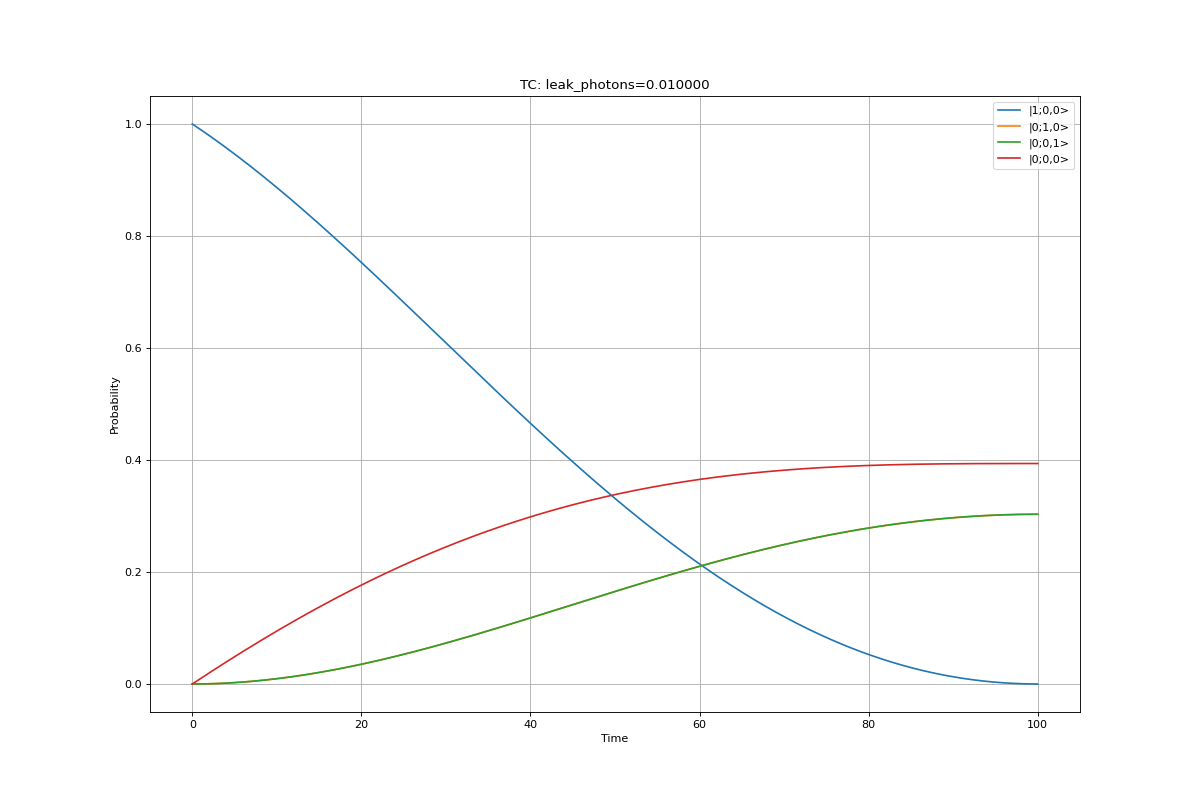
\includegraphics[width=0.9\paperwidth, height=0.4\textheight]{../examples/tc_example.png}}
			\caption{\label{tc_example} Вероятности состояний H\_TC.}
        \end{figure}

        У данного способа есть серьёзный недостаток - графики генерируются не параллельно, поэтому его можно использовать как для быстро отладки программы. Для серьёзных же вычислений рекомендую 
        использовать способ Seaborn.

        \subsection{Seaborn. Файловая система.}

        Второй способ работает с файловой системой (к слову, он работает и на версиях с Python API). Все результаты сохраняются в ФС в виде CSV файлов. Они устроены строго определённым образом и 
        гибкости там нет и не планируется в ближайшее время. Все эти файлы потом читаются с помощью вспомогательного скрипта, который после установки библиотеки
        будет хранится по пути \textsf{\$SEABORN\_PLOT}.
        Это питоновский скрипт, делающий графики с помощью пакета \textsf{seaborn}.
        Скрипт способен генерировать сразу несколько графиков одновременно, что удобно, например, для генерации gif изображений.
        У данного способа куда большая гибкость в кастомизации графиков, настройка которых происходит, собственно,
        с помощью конфигурационного файла, лежащего по пути \textsf{\$SEABORN\_CONFIG}. Объясняю, 
        как это всё работает.

        При записи графиков в ФС создаётся директория, которая потом будет названием этого графика. В него записывается 4 файла - вероятности (\textsf{probs.csv}),
         время (\textsf{time.csv}), гамильтониан (\textsf{hamiltonian.csv}), строковое представление базиса (\textsf{basis.csv}).

        Приведу пример (\textsf{blocked\_realization\_tc\_example.cpp}):

\begin{mdframed}[linecolor=black, topline=true, bottomline=true,
leftline=false, rightline=false]
\begin{minted}[mathescape]{c++}
std::vector<std::pair<double, OpType>> dec;
OpType A_out(a_destroy);
dec.emplace_back(state.get_leak(), A_out);

int ctxt;
mpi::init_grid(ctxt);

BLOCKED_H_by_Operator<TC_State> H(ctxt, state, H_op, dec);

auto time_vec = linspace(0, 1000, 1000);

auto probs = quantum_master_equation(state, H, time_vec);

// "seaborn_results/tc_example_seaborn" имя директории,
// в которую буду записаны файлы
// ВНИМАНИЕ! Если директория уже существует, она будет удалена!
// Рекомендуется записывать файлы в отдельную директорию
make_probs_files(H, probs, time_vec, H.get_basis(), "tc_example_seboarn");
\end{minted}
\end{mdframed}

        По итогу у нас созданы файл в директории \textsf{tc\_example\_seaborn}. Перейдём в директорию \textsf{seaborn\_results}.

        Теперь откроем \textsf{\$SEABORN\_CONFIG}. Это файл формата json, настраивающий работу скрипта.

\begin{mdframed}[linecolor=black, topline=true, bottomline=true,
leftline=false, rightline=false]
\begin{minted}[mathescape]{json}
{
    "format": "png", // Формат файла. Либо gif либо png.
    "filename": "filename", // название файла для результата gif
    "width": "19", // Ширина файла (в 100 пикселях)
    "height": "10", // Высота графика (в 100 пикселях)
    "dirs": "*", // Какие директории нужно обработать, выбор происходит также
                // как в линуксе
    "frames": "20", // Если выбран гиф - количество кадров
    "interval": "100" // Время в миллисекундах, с которой сменяется кадр
}
\end{minted}
\end{mdframed}

        Запустим этот скрипт с такими настройками - получим файл \textsf{tc\_example\_seaborn.png}.

        \begin{figure}[H]
			\makebox[\textwidth]{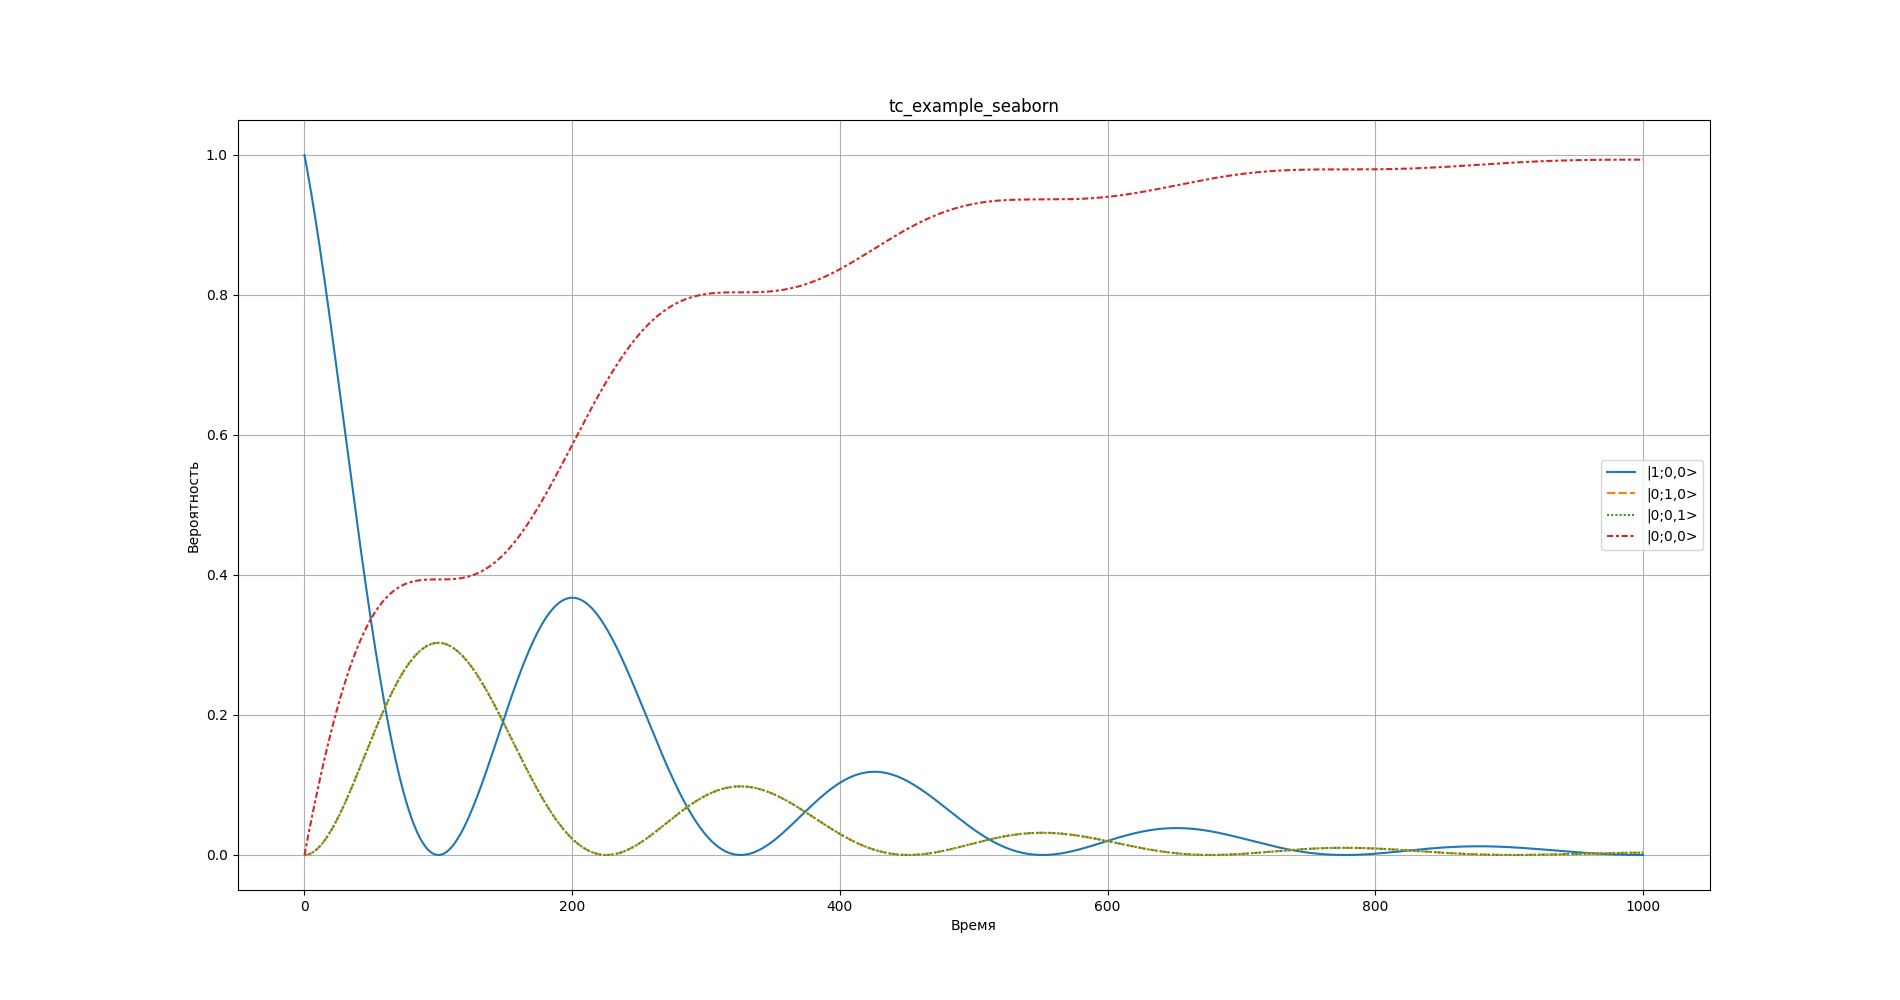
\includegraphics[width=0.9\paperwidth, height=0.4\textheight]{../examples/seaborn_results/tc_example_seaborn.png}}
			\caption{\label{tc_example_seaborn} Вероятности состояний H\_TC.}
        \end{figure}

        Данный способ допускает параллелизацию при генерации gif изображений, внутри генерации одного графика также параллелизации нет, что для больших графиков является проблемой, для которой 
        в ближайшее время решение не будет.

        Собственно, теперь давайте сделаем gif изображения, сделав перебор по интенсивности утечки фотонов для начального состояния $|0;1\rangle$. Файл - \textsf{gif\_tc\_example.cpp}.

\begin{mdframed}[linecolor=black, topline=true, bottomline=true,
leftline=false, rightline=false]
\begin{minted}[mathescape]{c++}
size_t steps_count = 500;
double a = 0.01, b = 0.15;
auto g_leak_range = linspace(a, b, steps_count);

size_t start, count;
make_rank_map(g_leak_range.size(), rank, world_size, start, count);

auto time_vec = linspace(0, 1000, 1000);

for (size_t i = start; i < count + start; i++) {
    auto g_leak = g_leak_range[i];
    state.set_leak(g_leak);
    H_TC H(state);

    auto probs = quantum_master_equation(state, H, time_vec);

    make_probs_files(H, probs, time_vec, H.get_basis(),
                     "gif_results/tc_g_leak=" + std::to_string(g_leak), rank);
}
\end{minted}
\end{mdframed}    

    Далее переходим в директорию \textsf{gif\_results}. Дальше настраиваем \textsf{\$SEABORN\_CONFIG} следующим образом:

\begin{mdframed}[linecolor=black, topline=true, bottomline=true,
leftline=false, rightline=false]
\begin{minted}[mathescape]{json}
{
    "format": "gif", // Формат файла. Либо gif либо png.
    "filename": "tc_gif.gif",
    "width": "19", // Ширина файла (в 100 пикселях)
    "height": "10", // Высота графика (в 100 пикселях)
    "dirs": "*", // Какие директории нужно обработать, выбор происходит также
                // как в линуксе
    "frames": "500", // Если выбран гиф - количество кадров
    "interval": "100" // Время в миллисекундах, с которой сменяется кадр
}
\end{minted}
\end{mdframed}

    Прописываем в командную строку \textsf{\$SEABORN\_PLOT} и готово! (Вес файла очень большой, поэтому его нет в репозитории.)

        \section{Инструкция к параллелизации}

        Мы прошли все основные этапы, связанные с данной библиотекой.
        Теперь я хочу дать некоторые практические советы по использованию и параллелизации. Дело в том, что квантовые вычисления в смысле 
        моделирования крайне неустойчивы к условию задачи - малейшие изменения (банальное изменение размерностей) могут заставить в корне поменять подход к паралеллизации.

        Ни одна библиотека не сможет решить абсолютно все подобные проблемы,
        ибо подобных нюансов слишком много, поэтому некоторые стратегии параллелизации придётся менять. Например, паралеллить вручную
        (хоть и не на самом низком уровне, благодаря библиотеке, а, например, по пачке гамильтонианов с разными параметрами).

        \subsection{Эффективные параметры запуска для основного квантового уравнения}

        Практика показывает, что параллельное перемножение матриц на нитях сильно выигрывает, 
        по сравнению с версиями на ядрах в силу огромного количества коммуникационных расходов последнего, а также синхронизаций. 
        Отсюда следующая рекомендация - запускать по 1 ядру на 1 узле. Данная конфигурация будет максимально эффективной.

        Для \textbf{schrodinger} данные рассуждения не работают (на данный момент, в будущем будет переделано),
        для него наоборот - наиболее эффективным будет большое число ядер (не больше размерности базиса, разумеется).
        
        \subsection{Маленькие базисы}

        При маленьком размере блоков (NB, MB <= 64) вместо ускорения при параллельном перемножении, вы получите сильное замедление. 

        Многоядерная версия \textbf{QComputations} является расширением одноядерной версии, то есть,
        всё, что есть в одноядерной версии, есть и в многоядерной, что позволяет параллелить вручную одноядерную. Для 
        этой цели в библиотеке реализованы вспомогательные функции. (Все они перечислены в документации в главе \textsf{Вспомогательные функции})

        Пример решения этой проблемы уже был показан - \textsf{gif\_tc\_example.cpp}. Там размер гамильтониана равен 4.
        
\end{document}